\documentclass[../TDE8_filtrage.tex]{subfiles}%

\begin{document}
\section[s]"2"{Filtre ADSL}
\enonce{%
	Un lutin malin semble avoir chourré votre filtre ADSL. Sale histoire.
	Heureusement, vous avez les connaissances pour en recréer un~! En sachant que
	les signaux transmis par une ligne téléphonique utilisent une très large gamme
	de fréquences, divisée en deux parties~:
	\begin{itemize}
		\item les signaux téléphoniques (transmettant la voix) utilisent les
		      fréquences de 0 à \SI{4}{kHz}~;
		\item les signaux informatiques (Internet) utilisent les fréquences de
		      \SI{25}{kHz} à \SI{2}{MHz}.
	\end{itemize}
}

\QR{%
	Quel type de filtre faut-il utiliser pour récupérer seulement les
	signaux téléphoniques~? Les signaux informa- tiques~? Quelle fréquence
	de coupure peut-on choisir~?
}{%
	On isole les signaux téléphoniques avec un \textbf{filtre passe-bas},
	et les signaux informatiques avec un \textbf{filtre passe-haut}. La
	fréquence de coupure doit être à la fois nettement supérieure aux
	fréquences téléphoniques et nettement plus faible que les fréquences
	informatiques~: on prendra donc \fbox{$f_0 = \SI{10}{kHz}$}.
}

\enonce{%
	Vous réalisez le filtre ci-dessous.
	\begin{center}
		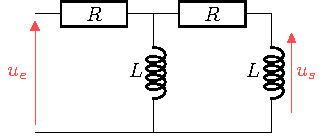
\includegraphics[width=.5\linewidth]{adsl_plain}
	\end{center}
}

\QR{%
	Déterminer la nature du filtre grâce à son comportement asymptotique
	en basses fréquences et en hautes fréquences. En déduire pour quels
	signaux il peut être utilisé.
}{%
	~
	\vspace{-15pt}
	\smallbreak
	\noindent
	\begin{isd}
		En basses fréquences ($\w \to 0$), les bobines se
		comportent comme des fils, soit
		\begin{center}
			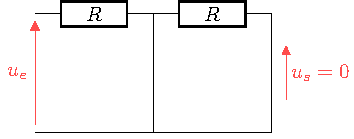
\includegraphics[width=\linewidth]{adsl_bf}
		\end{center}
		\tcblower
		En hautes fréquences ($\w \to \infty$), les bobines se
		comportent comme des interrupteurs ouverts, soit
		\begin{center}
			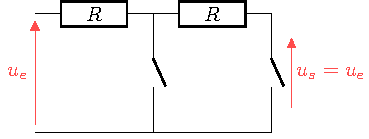
\includegraphics[width=\linewidth]{adsl_hf}
		\end{center}
	\end{isd}
	Ainsi, le signal de sortie est non nul pour les hautes fréquences, et
	négligeable pour les basses fréquences~: c'est un \textbf{filtre
		passe-haut}. Il permettra d'obtenir les signaux informatiques.
}

\QR{%
	Montrer que la fonction de transfert de ce filtre peut se mettre sous
	la forme~:
	\[\Hu(x) = \frac{-x^2}{1 + 3\jx-x^2}
		\qavec
		x = \frac{\w}{\w_0}
	\]
	et exprimer $\w_0$ en fonction de $R$ et $L$.
}{%
	Pour exprimer $u_s$ en fonction de $u_e$, on peut faire un premier
	pont diviseur de tension pour exprimer $u_s$ en fonction de $u_{AB}$ du
	milieu~; puis avec une impédance équivalente à l'ensemble des 3 dipôles
	de droite, on refait un pont diviseur de tension pour avoir $u_{AB}$ en
	fonction de $u_e$, et on combine.
	\begin{center}
		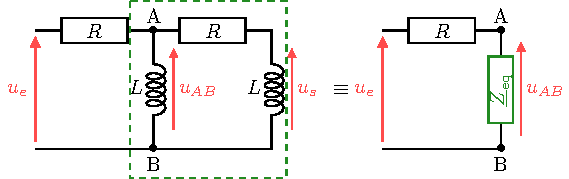
\includegraphics[width=0.8\linewidth]{adsl_equiv}
	\end{center}
	On a donc d'abord~:
	\begin{gather*}
		\Uu_s = \frac{\Zu_L}{\Zu_L + \Zu_R}\Uu_{AB}
		\Lra
		\Uu_s = \frac{\jlw}{\jlw + R}\Uu_{AB}
	\end{gather*}
	On aura donc ensuite~:
	\begin{gather*}
		\Uu_{AB} = \frac{\Zu\ind{eq}}{\Zu\ind{eq} + \Zu_R}\Uu_e
		\Lra
		\Uu_{AB} = \frac{1}{1+\Zu_R\Yu\ind{eq}}\Uu_e
	\end{gather*}
	On calcule alors $\Yu\ind{eq}$~:
	\begin{gather*}
		\Yu\ind{eq} = \frac{1}{\jlw} + \frac{1}{R+\jlw}
	\end{gather*}
	Et on combine~:
	\begin{gather*}
		\Uu_s =
		\frac{\jlw}{R+\jlw}\times\frac{1}{1+\Zu_R\Yu\ind{eq}}\Uu_e
		\Lra
		\Uu_s =
		\frac{\jlw}{R + \jlw + R \left( \dfrac{R+\jlw}{\jlw} + 1
			\right)}\times {\color{Red} \frac{\jlw}{\jlw}}\Uu_e\\
		\Lra
		\Uu_s =
		\frac{-(L\w)^2}{R^2 + 3\jj RL\w - (L\w)^2}\Uu_e
		\Lra
		\Uu_s =
		{\color{red}\cancel{\frac{R^2}{R^2}}}
		\frac{- \left( \dfrac{L}{R}\w \right)^2}{1 + 3\jj \dfrac{L}{R}\w
			- \left( \dfrac{L}{R}\w \right)^2}
		\Uu_e
	\end{gather*}
	Ainsi, en divisant par $\Uu_e$ pour avoir la fonction de transfert, on
	a~:
	\begin{gather*}
		\boxed{\Hu = \frac{-x^2}{1-x^2+3\jx}}
		\qavec
		\boxed{\w_0 = \frac{R}{L}}
	\end{gather*}
}

\QR{%
Tracer le diagramme de Bode asymptotique (gain et phase) de ce filtre,
puis esquisser l'allure de la courbe réelle de gain en la justifiant.
}{%
Pour $x \gg 1$, les termes en $x^2$ l'emportent sur les autres termes
au numérateur et au dénominateur, et la fonction de transfert devient
$\Hu \underset{x\ra\infty}{\sim} 1$, donc \fbox{$G_{\dB} = 0$}
et \fbox{$\f = 0$} (réel positif).
\bigbreak
Pour $x \ll 1$, les termes en $x$ sont négligeables devant $1$ au
dénominateur, et on garde le numérateur~: la fonction de transfert
devient donc $\Hu \underset{x\ra0}{\sim} -x^2$, donc
\fbox{$G_{\dB} \underset{x\ra0}{\sim} 40\log(x)$} (pente de
\SI{40}{dB/décade}).
Pour la phase, c'est moins évident, on pourrait avoir $\f = \pm \pi$ puisque
c'est un réel négatif. Il faut étudier le domaine d'existence $\forall x$~:
\begin{DispWithArrows*}
	\arg*{\Hu(x)} &= \arg*{-x^2} - \arg*{1-x^2 + 3\jx}
	\Arrow{$-\arg*{\zu} = \arg*{\zu^*}$}
	\\
	&= \arg*{-x^2} + \arg*{\pa{1-x^2 - 3\jx}\frac{\jj }{\jj }}
	\Arrow{$\arg*{\frac{\zu_1}{\zu_2}} = \arg*{\zu_1} - \arg*{\zu_2}$}
	\\
	&= \underbracket[1pt]{\arg*{-x^2}}_{\pm \pi} +
	\underbracket[1pt]{%
	\underbracket[1pt]{\arg*{3x + \jj \pa{1-x^2}}}_{%
	\in \left] - \frac{\pi}{2}\,; \frac{\pi}{2} \right[
	} -
	\underbracket[1pt]{\arg*{\jj }}_{\frac{\pi}{2}}
	}_{\in \left] -\pi\,; 0 \right[}
\end{DispWithArrows*}
Ainsi, pour que l'angle s'exprime entre $\left] -\pi\,;\pi \right[$, on a
forcément $\arg*{-x^2} = +\pi$, soit \fbox{$\f = \pi$}.
\bigbreak
Pour $x = 1$, on trouve $\Hu(1) = \jj/3$ donc \fbox{$G_{\dB}(1) =
		20\log(1/3) = \SI{-9.5}{dB}$}, et \fbox{$\f(1) = \pi/2$} (imaginaire pur).
\begin{center}
	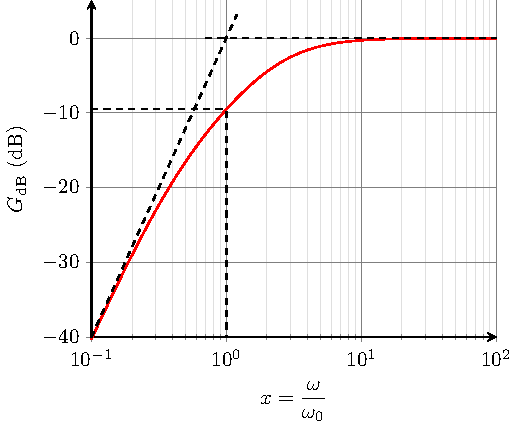
\includegraphics[width=.48\linewidth]{adsl_bode-gain}
	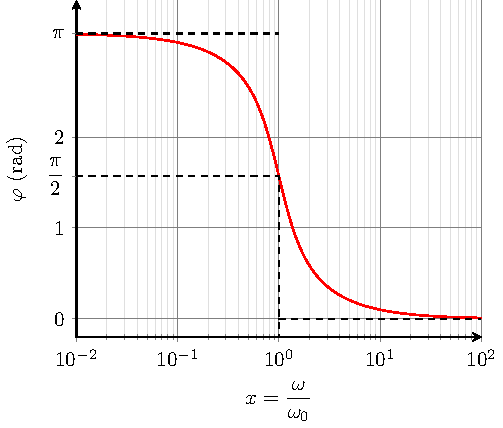
\includegraphics[width=.48\linewidth]{adsl_bode-phase}
\end{center}
Il n'y a pas de pic de résonance car le facteur de qualité $Q$ est
plus petit que $1/\sqrt{2}$.
}

\QR{%
	Vous possédez des résistances de $\SI{100}{\Omega}$. Quelle valeur
	d'inductance $L$ choisir pour réaliser le filtre souhaité~?
}{%
	La fréquence de coupure est $f_0 = \DS \frac{\w_0}{2\pi} =
		\frac{R}{2\pi L}$~; on doit donc prendre
	\begin{gather*}
		\boxed{L = \frac{R}{2\pi f_0}}
		\qavec
		\left\{
		\begin{array}{rcl}
			R   & = & \SI{100}{\Omega} \\
			f_0 & = & \SI{10}{kHz}
		\end{array}
		\right.\\
		\mathrm{A.N.~:}\quad
		\boxed{L = \SI{1.6}{mH}}
	\end{gather*}
}
\end{document}
